\documentclass[11pt,reqno]{amsart}
\usepackage{geometry}                % See geometry.pdf to learn the layout options. There are lots.
\geometry{letterpaper}                   % ... or a4paper or a5paper or ... 
\usepackage[parfill]{parskip}    % Activate to begin paragraphs with an empty line rather than an indent
\usepackage{algorithm, algorithmic}
\usepackage{graphicx}
\usepackage{natbib}
\usepackage{amssymb}
\usepackage{amsmath}
\usepackage{pdfpages}
\usepackage{subfig}
\usepackage{enumitem}
\usepackage[skip=2pt,font=scriptsize]{caption}
\newcommand{\RR}{I\!\!R} %real numbers
%\usepackage{epstopdf}
%\DeclareGraphicsRule{.tif}{png}{.png}{`convert #1 `dirname #1`/`basename #1 .tif`.png}


\DeclareMathOperator{\diag}{diag}

\title[RVD2: Supplementary Information]{Supplementary Information for
  RVD2: An ultra-sensitive variant detection model for low-depth heterogeneous next-generation sequencing data}
%\date{}      % Activate to display a given date or no date

\begin{document}
\maketitle

%%%%%%%%%%%%%%%%%%%
% Appendix A: An simulation example to illustate the idea of proposal graphical model and v.
%%%%%%%%%%%%%%%%%%%
\section{Example to illustrate the proposal graphical model and generative process.}\label{sec:appendix_example}

\begin{figure}[!bpth]
    \centering
    \subfloat[\label{fig:example:a}]{{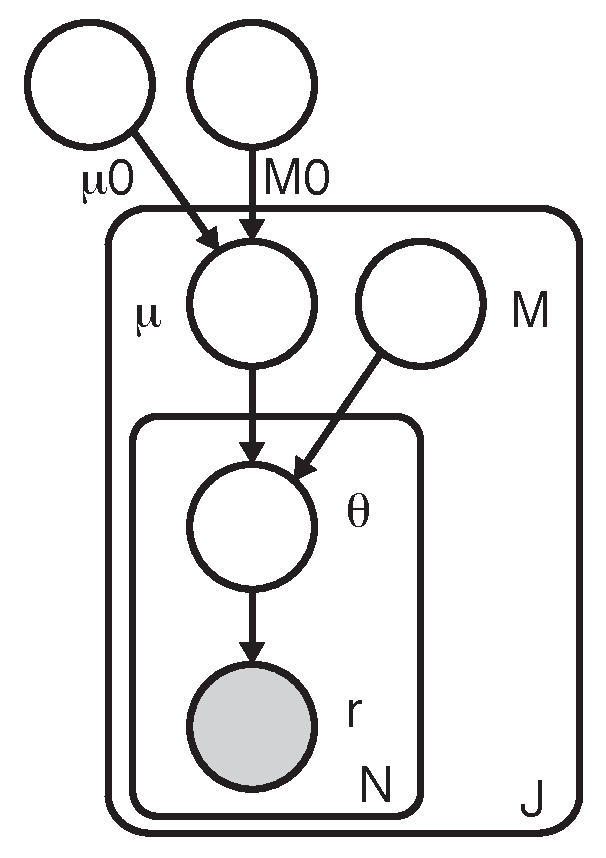
\includegraphics[width=0.2\textwidth]{pdf_figs/RVD2_model.pdf} }}%
    \quad
    \quad
    \subfloat[ \label{fig:example:b}]{{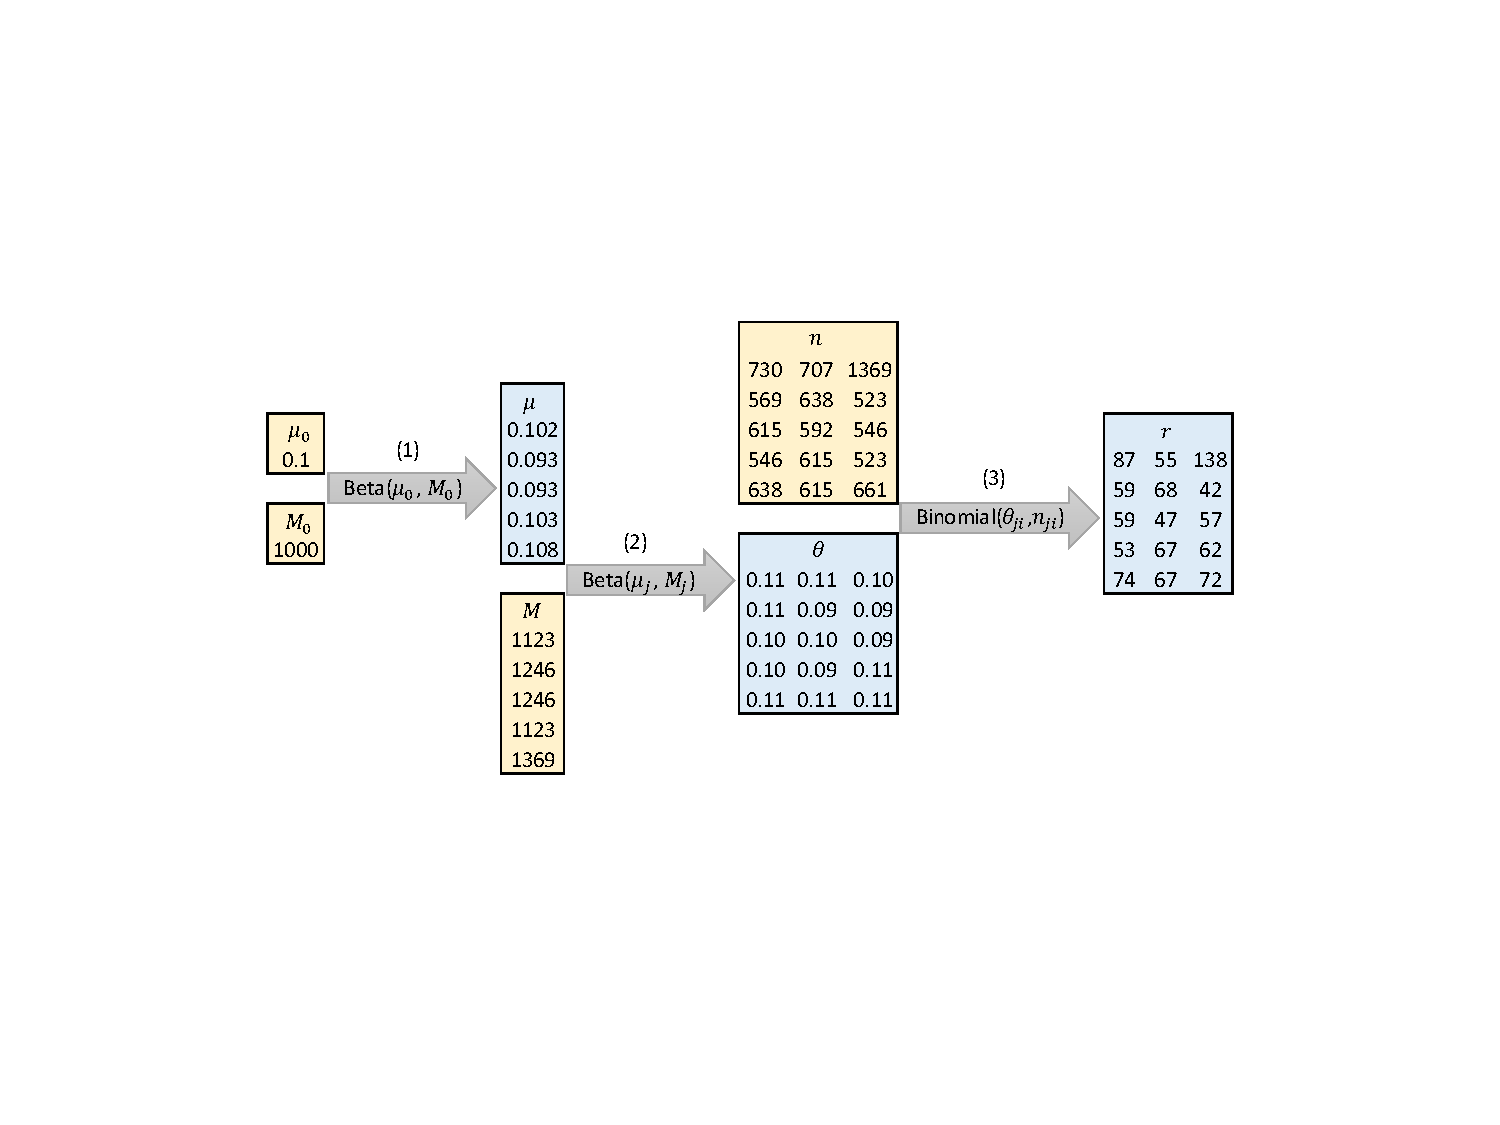
\includegraphics[width=0.7\textwidth]{pdf_figs/GMexample.pdf} }}%
    \caption{(A) RVD2 Graphical Model. (B) Example to illustrate the proposal graphical model and generative process. Here we want to generate a simulation sample with 3 replicates, and each replicate is a 5bp long sequence. Therefore, we have $ J = 5 $, $N = 3$. The hyperparameters in orange, $\mu_0 \in \RR^{1 \times 1}$, $M_0 \in \RR^{1 \times 1}$, $M \in \RR^{5 \times 1}$ are set. $n \in \RR^{5 \times 3}$ in the generative process is given as well. The generative process is: (1) Sample the local error rate $\mu \in \RR^{5 \times 1}$ by drawing random numbers $\mu_j \thicksim \text{Beta}(\mu_0, M_0)$. (2) Use $\mu $ and $ M $ to sample $\theta \in \RR^{5 \times 3}$ by drawing random samples $\theta_{ji} \thicksim \text{Beta}(\mu_j, M_j)$. (3) Use $\theta \in \RR^{5 \times 3}$ and $n \in \RR^{5 \times 3}$ to sample $r \in \RR^{5 \times 3}$ by drawing random numbers $r_{ji} \thicksim \text{Binomial}(\theta_{ji}, n_{ji})$.} 
    \label{fig:example}
\end{figure}

%%%%%%%%%%%%%%%%%%%
% Appendix A: Parameter Initialization
%%%%%%%%%%%%%%%%%%%
\section{Parameter Initialization}\label{sec:appendix_mom}
Since $r_{ji} \thicksim \text{Binomial}(n_{ji}, \theta_{ji})$, the first population moment is  $E[r_{ji}] = \theta_{ji} n_{ji}$ and the first sample moment is simply $m_1 = r_{ji}$. Therefore the MoM estimator is
\begin{equation}
	\hat{\theta}_{ji} = \frac{r_{ji}} {n_{ji}}
\end{equation}

We take the MoM estimate, $\hat{\theta}_{ji}$, as data for the next conditional distribution in the hierarchical model. The distribution is $\theta_{ji} \thicksim \text{Beta}(\mu_jM_j, (1-\mu_j)M_j)$. The first and second population moments are
\begin{eqnarray}
	E[\theta_{ji}] =& \mu_j,\\
	\text{Var}[\theta_{ji}] =& \frac{\mu_j(1-\mu_j)} { M_j + 1 }.
\end{eqnarray}
The first and second sample moments are $m_1 = \frac{1}{N}\sum_{i=1}^N \theta_{ji}$ and $m_2 = \frac{1}{N}\sum_{i=1}^N \theta_{ji}^2$. Setting the population moments equal to the sample moments and solving for $\mu_j$ and $M_j$ gives
\begin{eqnarray}
	\hat{\mu}_j =& \frac{1}{N} \sum_{i=1}^N \hat{\theta}_{ji}, \\
	\hat{M_j} =& \frac{ \hat{\mu}_j (1 - \hat{\mu}_j ) } { \frac{1}{N} \sum_{i=1}^N \hat{\theta}_{ji}^2 } -1.
\end{eqnarray}

Following the same procedure for the parameters of $\mu_j \thicksim \text{Beta}(\mu_0, M_0)$ gives the following MoM estimates
\begin{eqnarray}
	\hat{\mu}_0 =& \frac{1}{J} \sum_{j=1}^J \hat{\mu}_j \\
	\hat{M}_0 =& \frac{ \hat{\mu}_0 (1 - \hat{\mu}_0 ) } {\frac{1}{J} \sum_{j=1}^J \hat{\mu}_j^2 } -1.
\end{eqnarray}



%%%%%%%%%%%%%%%%%
% Appendix B: Data Set Statistics
%%%%%%%%%%%%%%%%%
\section{RVD2 Estimated Parameters}\label{sec:synthetic_estimate}
The RVD2 algorithm provides estimates of model parameters and latent variables given the data. We show several of these parameters in Figure~\ref{fig:depthM}.

\begin{figure}[htbp]
\begin{center}
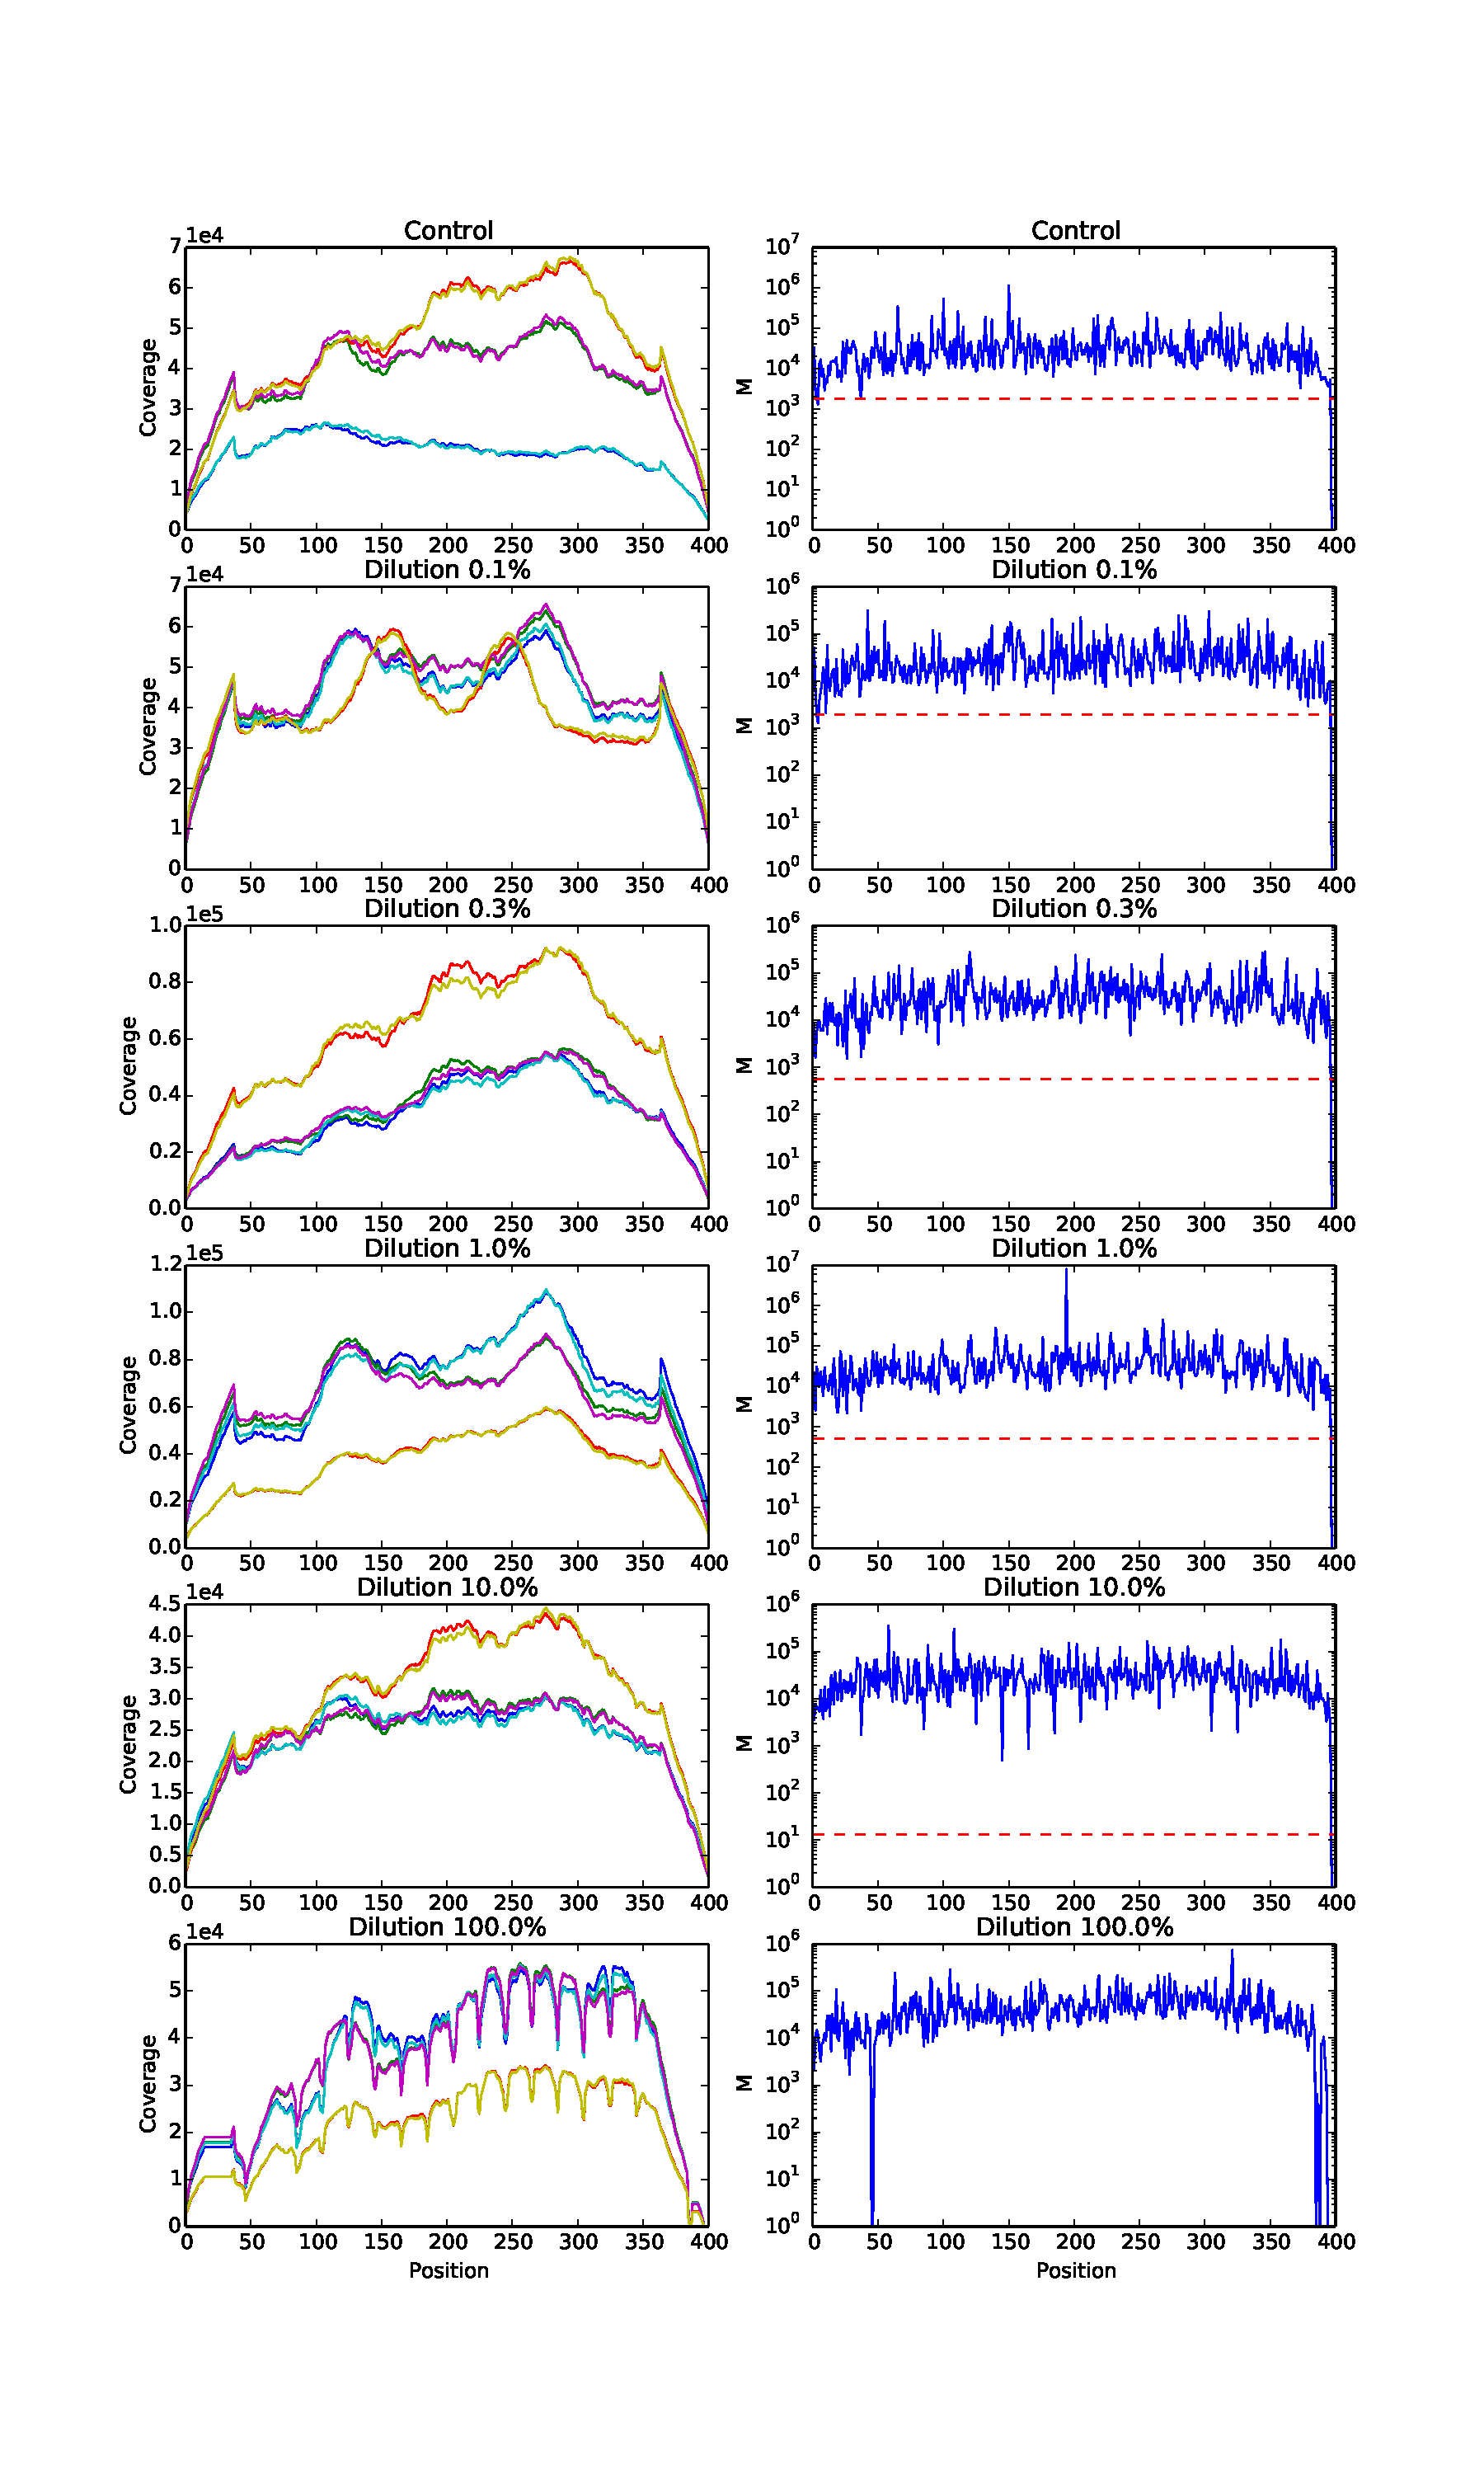
\includegraphics[width=0.85\textwidth]{pdf_figs/depthM.pdf}
\caption{Key parameters for RVD2 model for synthetic DNA data sets.}
\label{fig:depthM}
\end{center}
\end{figure}

The left column of Figure~\ref{fig:depthM} shows the read depth for each of the six bam files (three replicates each with two read pairs) for each data set. Because the DNA was not sheared and ligated prior to sequencing, the read depth drops to zero at the boundaries. For the 100\% mutant data set, the read depth drops at the mutant locations. This is due to the parameters imposed at the alignment stage. The reads are 36bp long and we required no more than 2 mismatches. Therefore, reads that overlapped two mutations (spaced 20bp apart by design) and included one additional mutation would not align.



% from folder '22013-11-15_depthM_plot_avg10', dilution rate is 0.1.

The right column of Figure~\ref{fig:depthM} shows the parameter estimates $\hat{M}_j$ and $\hat{M}_0$ for each data set. $M_j$ measures the variance between replicates at location $j$. There is little variability across positions indicating that the replication variance does not change greatly across position. 

%Furthermore, we see that $M_j$ does not change with read depth (except where the depth goes to zero) indicating that $M_j$ because $M_j$ is capturing a different process than the read depth.

The error rate across positions is captured by the $M_0$ parameter shown as a horizontal dotted line in the plots in the right column. We see that the variation between replicates is smaller than the variation between location. $M_j$ and $M_0$ are precision parameters, they are inversely proportional to the variance. Where $M_j$ is greater than $M_0$ the precision between replicates is higher than the precision across positions.

%%%%%%%%%%%%%%%%%%%
% Appendix C: Comparison Statistics
%%%%%%%%%%%%%%%%%%%
\section{Algorithm Comparison Statistics}\label{sec:app_comparison}
Figure~\ref{fig:comparison_mcc} compares RVD2 with samtools, GATK, varscan, strelka and muTect using Matthews Correlation Coefficient (MCC)~\citep{matthews1985homeostasis}.
\begin{figure}[ht]
\begin{center}
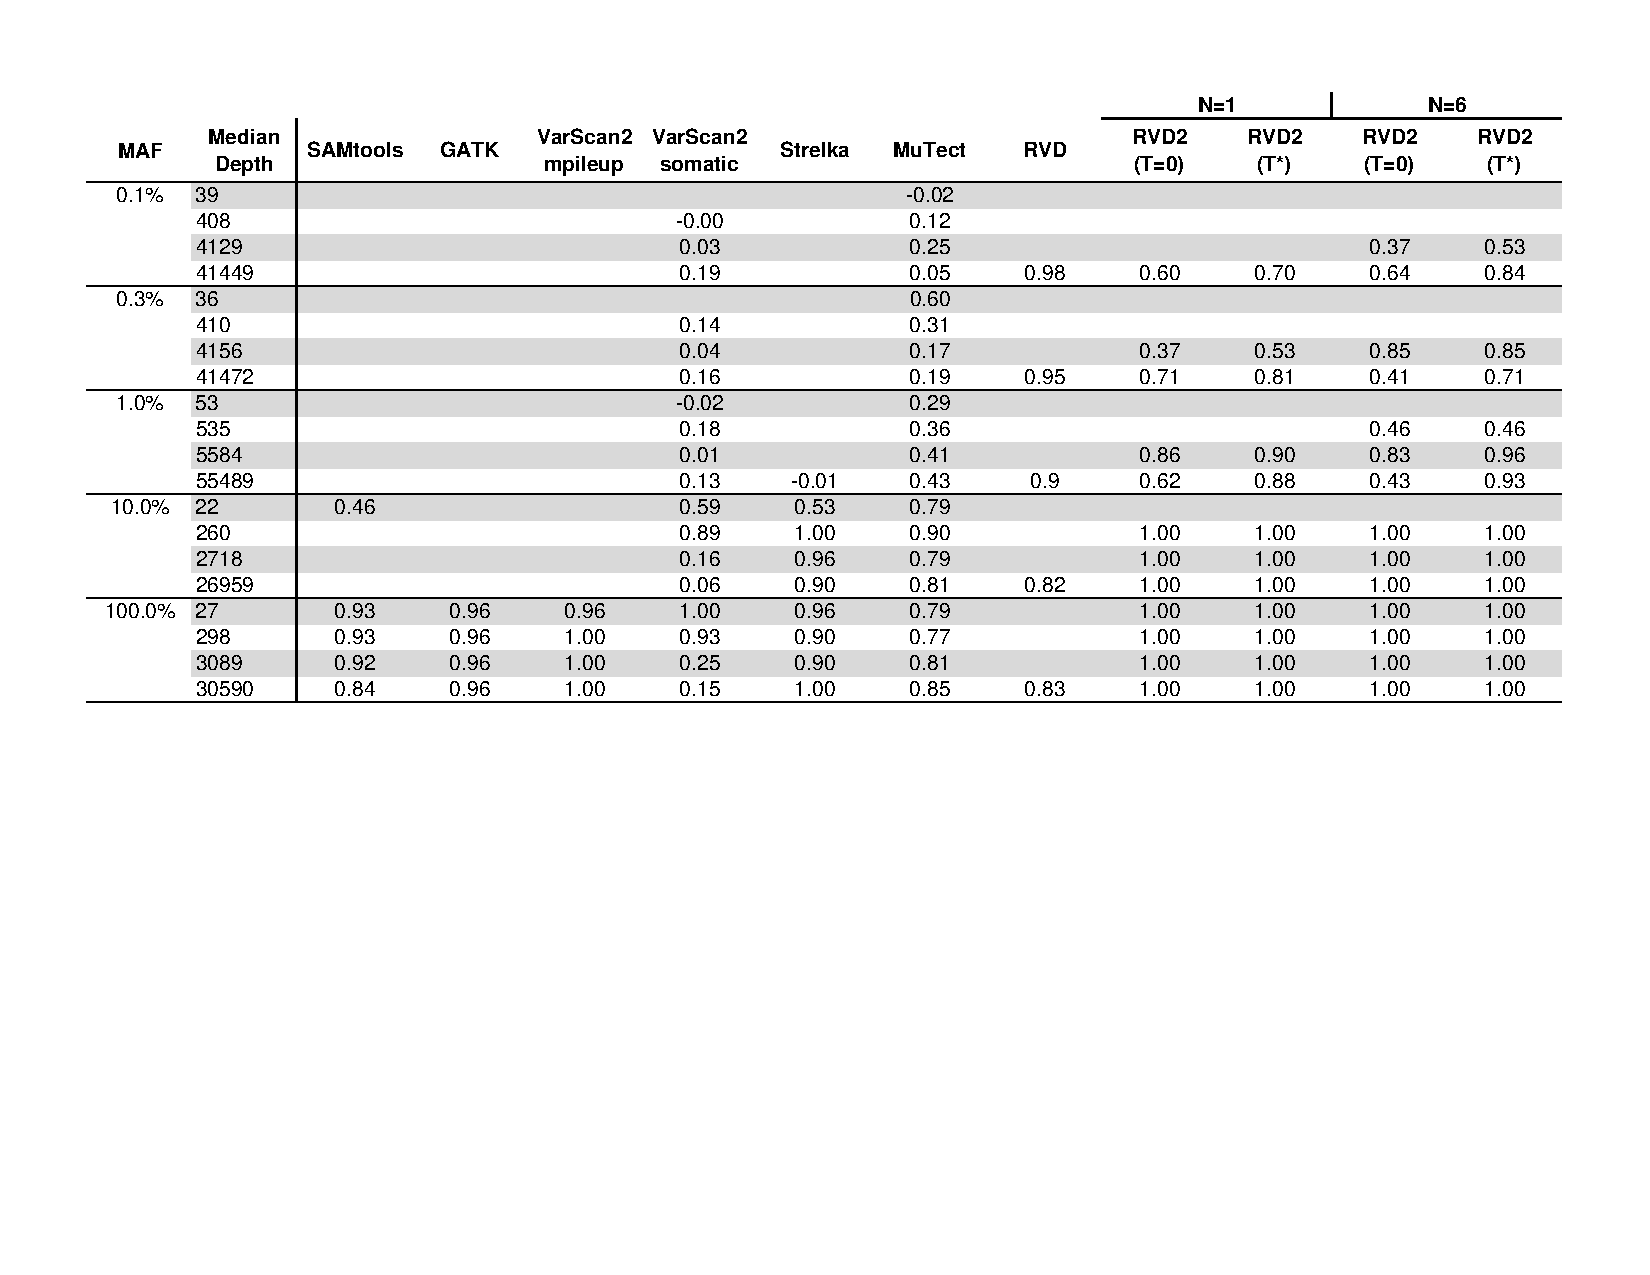
\includegraphics[width=1\textwidth]{pdf_figs/comparison_table_mcc.pdf}
\caption{Matthews correlation coefficient (MCC) comparison with other variant calling algorithms.}
\label{fig:comparison_mcc}
\end{center}
\end{figure}
% from folder 'rvd2\results\2013-09-19_operating_characteristics'
% from folder 'rvd2\results\2013-09-19_operating_characteristics'

Samtools and VarScan2-mpileup achieved MCC value generally higher than 0.90 on 100\% MAF sample across all read depthes, with 1.0 represents for a perfect prediction. However, both of them detected no variant when MAF is 10.0\% or lower, with only one exception for samtools when MAF is 10.0\% and read depth 22. GATK, Varscan2-somatic, Strelka and GATK outperformed Samtools and VarScan2-mpile on the 10.0\% MAF sample, while approximately tied in other cases. Strelka achieved best MCC on 10\% MAF sample comparing to Varscan2-somatic and GATK, more specifically around 1.00 when read depth is 260 or higher. There is a very obvious but unconventional decreasing trend in VarScan2-somatic MCC value across different read depth and MAF level, a phenomenon also observed by~\citealp{Stead:2013fu}. It is because VarScan2-somatic tends to call more false positives as read depth gets higher. Mutect seems to performs the best among all the algorithms expect RVD2 when MAF is 1.0\% or lower. It achieves MCC values varying from -0.02 to 0.43, though too low to be practically meaningful. However, muTect achieved relatively lower MCC values when the MAF level is 10\% and 100\%, as a counteractive of being oversensitive.

RVD2 achieved MCC value 1.00 when the MAF is 100.0\% at all read depth and 10\% when read depth is not lower than 260. This indicates that RVD2($\tau=0, N=1$) is more accurate than the other algorithms when the median read depth is at least $10\times$ the MAF.
%%%%%%%%%%%%%%%%%
% Appendix D: Estimated minor allele fraction for called variants in synthetic gene.
%%%%%%%%%%%%%%%%%
\section{Estimated MAF for called variants in synthetic gene.}
Figure~\ref{fig:MAF} shows the posterior mean and 95\% credible intervals for $\mu_j$ for called variant positions with $\bar{n} = 5584$ and MAF = 1.0\%. All of the called positions show a clear difference between the case and control error rates. The posterior mean estimates are all shrunken towards the global error rate parameter $\mu_0 = 0.0023$ due to the hierarchical structure of the model.
%
\begin{figure}[h]
\begin{center}
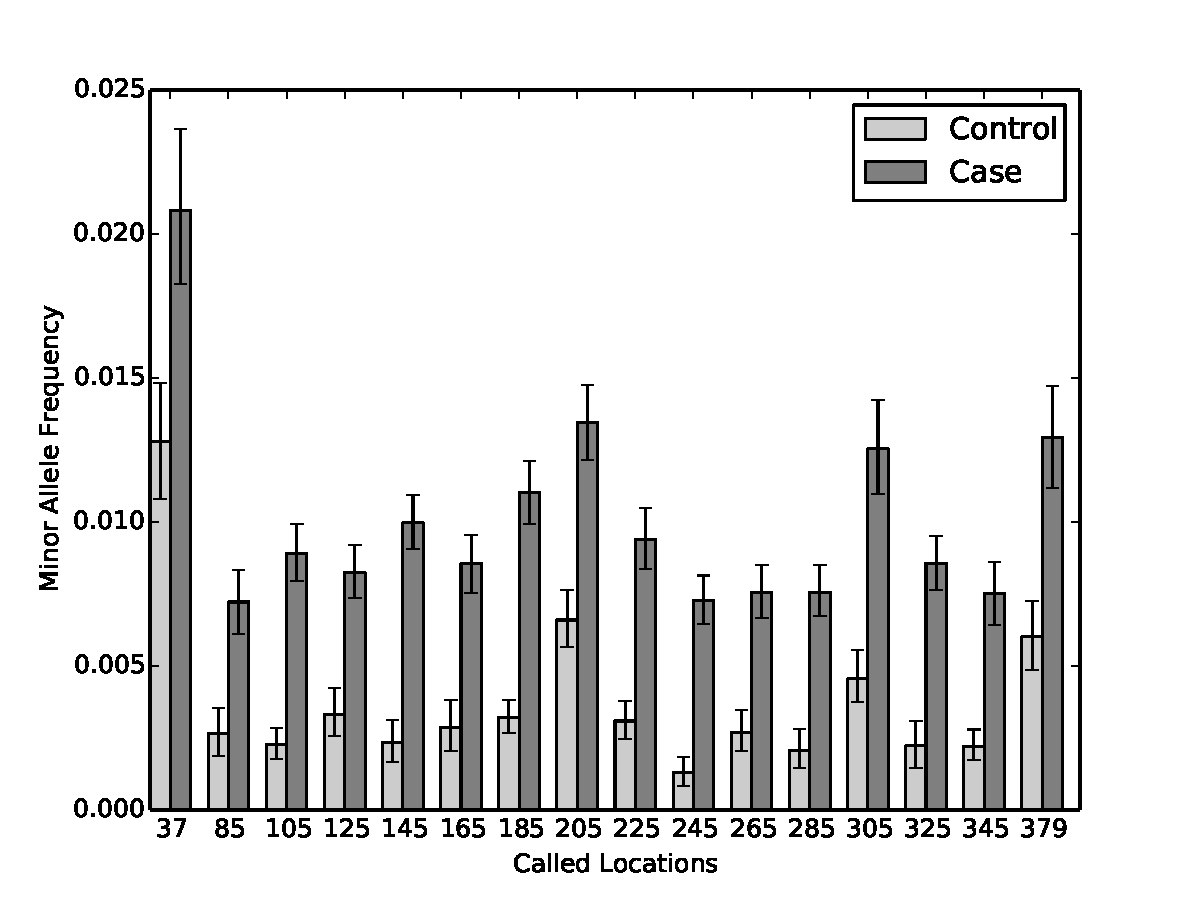
\includegraphics[width=1\textwidth]{pdf_figs/Synthetic_Mubarplot_MAF1_0_Depth5584.pdf}
\caption{Estimated minor allele fraction for called variants in 1.0\% dilution.}
\label{fig:MAF}
\end{center}
\end{figure}
% from folder '2013-11-15_synthetic_mu_barplot_optimalT', dilution rate is 0.1, downsampling rate is 0.01.


%%%%%%%%%%%%%%%%%
% Appendix E: Parameter Settings for Variant Calling Algorithms
%%%%%%%%%%%%%%%%%
\newpage
\section{Parameter settings for other variant calling algorithms}
\paragraph{\textbf{Samtools}}We used samtools (v0.1.19) function mpileup to call variants and bcftools to save the result in standard VCF files. In mpileup, we set the -d option sufficiently high at $10^6$ to avoid truncating read deapth. Option -u was enabled to make sure the output bcf files were uncompressed.

\paragraph{\textbf{GATK}}
We used GATK (v2.1-8) UnifiedGenotyper function to detect mutations on our synthetic data following the recommended workflow. Due to some format incompatibility, we applied Picard to format read group and GATK for realignment. In UnifiedGenotyper, -ploid (Number of samples in each pool $\times$ Sample Ploidy) was set at 1 because our synthetic data is haploid; -dcov was set at $10^6$ to avoid downsampling coverage within GATK.

\paragraph{\textbf{VarScan2-mpileup}}
VarScan2 (v2.3.4) mpileup2snp is a SNP calling program which takes multi-samples from samtools mpileup pipeline.We assigned parameter -C value 50 as the synthetic data was aligned using BWA and set -d at $10^6$. In mpileup2snp, --min-var-freq, the only non-default parameter, was set low enough at $10^{-5}$ because the variant frequency can be as low as $10^{-3}$.

\paragraph{\textbf{VarScan2-somatic}}
We tested VarScan2 somatic on our synthetic dataset. The parameter --normal-purity set was at 1.00, --tumor-purity at the dilution rate. The parameter --min-var-freq was set at $10^{-5}$. We combined all the positions VarScan2-somatic called regardless the somatic status (Germline/LOH/Somatic/Unknown) to compare with performance of RVD2.

\paragraph{\textbf{Strelka and muTect}}
Since configuration and Analysis for Strelka and muTect is standardized and no parameter needs to be specified, we installed these two programs and ran them on our data set separately.

Samtools mpileup and GATK can accept multiple tumor replicates for variant calling, so we fed six bam files from each case replicate group to mpileup. VarScan2-mpileup takes multiple tumor-normal pair replicates so we passed six pair replicates to each algorithm. Varscan2-somatic, strelka and muTect do not accept replicate data for the normal or tumor bam files so we used a single bam file from each replicate group with a read depth that most closely matched the overall median depth of the replicates.


\section{histogram of $ \hat{\mu}_j $ for somatic mutations called by rvd2 in the 44kbp paxip1 gene from chr7:154738059 to chr7:154782774 in hcc1187 dataset}
\begin{figure}[H]
\begin{center}
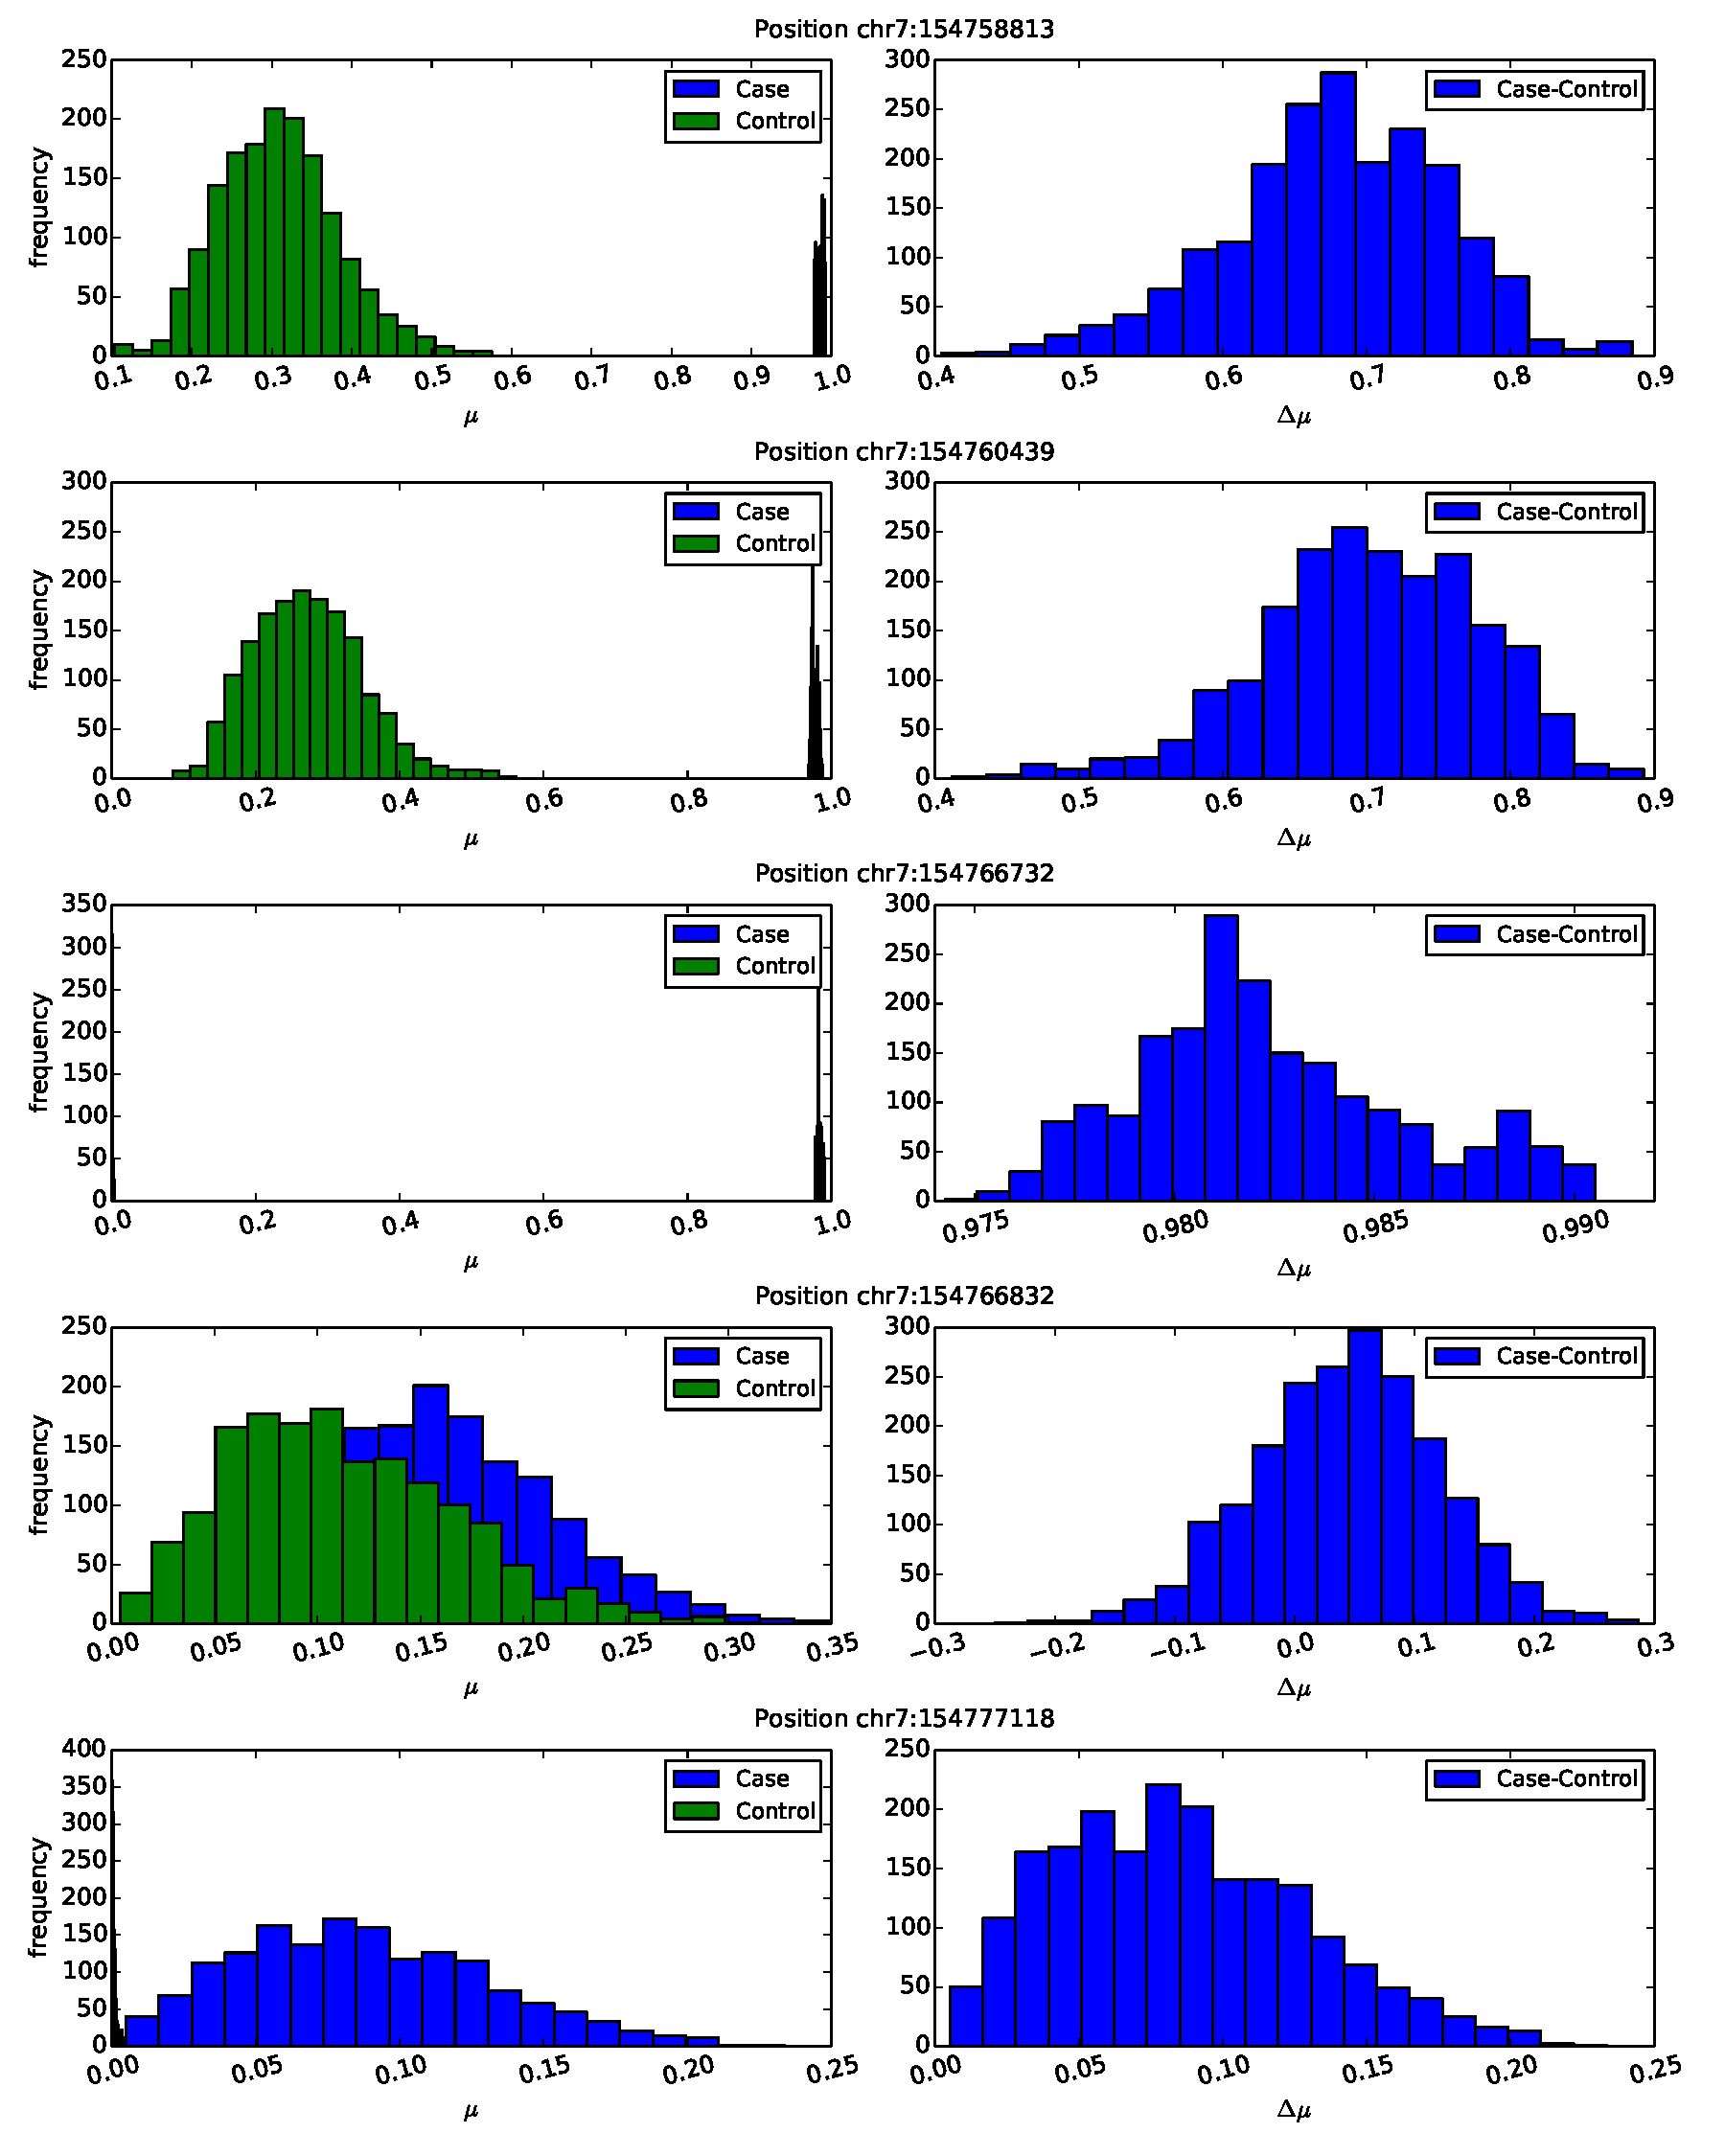
\includegraphics[width=1\textwidth]{pdf_figs/HCC1187_histogram_pos.pdf}
\caption{Histogram of $ \hat{\mu}_j $ for positions where $\mu^{\text{case}}$ is significantly higher than $ \mu^{\text{control}}$, namely Pr$ (\Delta \hat{\mu}_j> \tau) > 1- \alpha $, where $ \tau=0, \alpha=0.05 $.} 
\label{fig:hist_pos}
\end{center}
\end{figure}

\begin{figure}[H]
\begin{center}
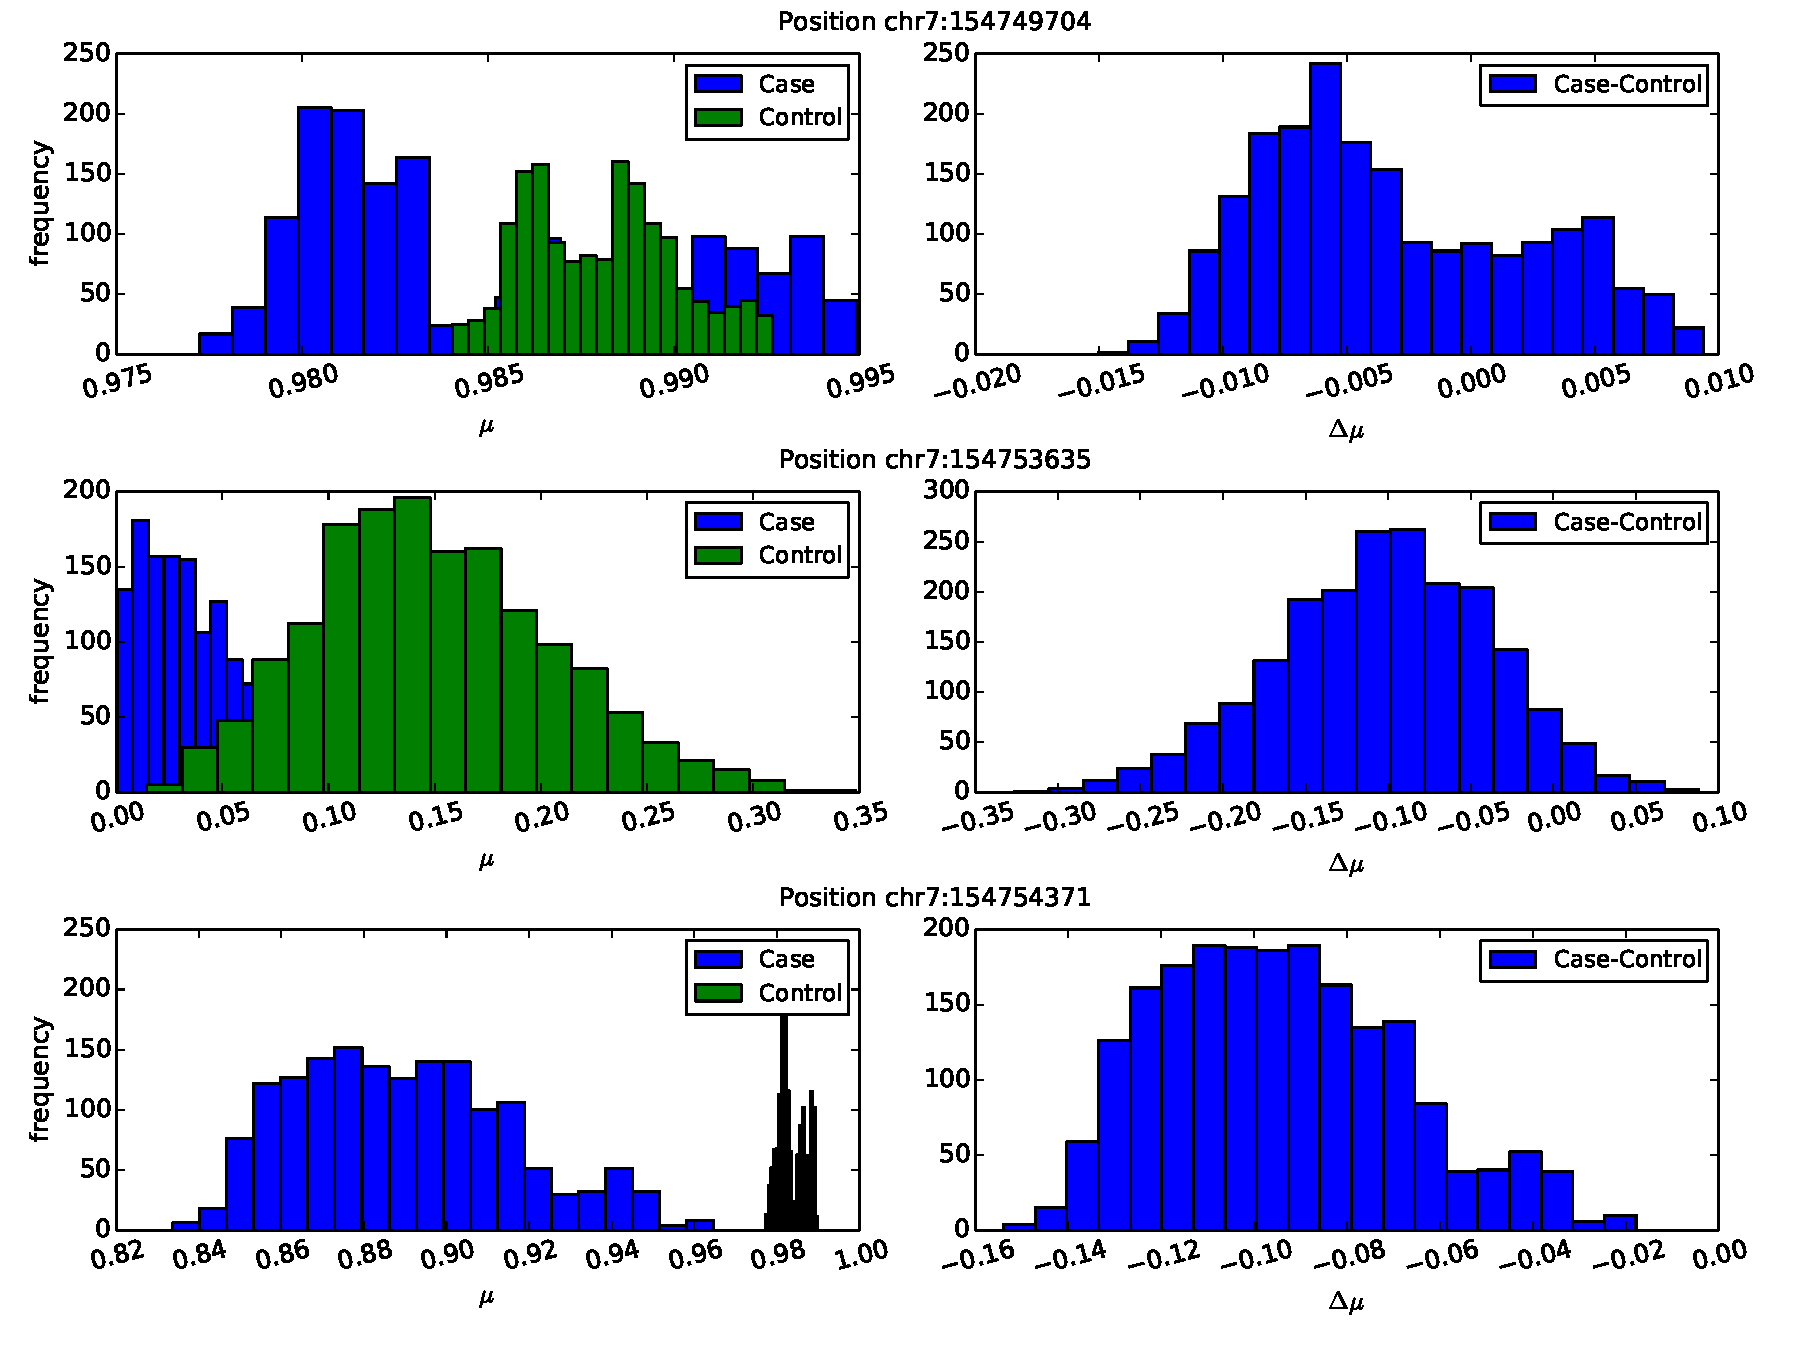
\includegraphics[width=1\textwidth]{pdf_figs/HCC1187_histogram_neg.pdf}
\caption{Histogram of $ \hat{\mu}_j $ for positions where $\mu^{\text{case}}$ is significantly lower than $ \mu^{\text{control}}$, namely Pr$ (\Delta \hat{\mu}_j< \tau) > 1- \alpha $, where $ \tau=0, \alpha=0.05 $.}
\label{fig:hist_neg}
\end{center}
\end{figure}

\bigskip
\bigskip


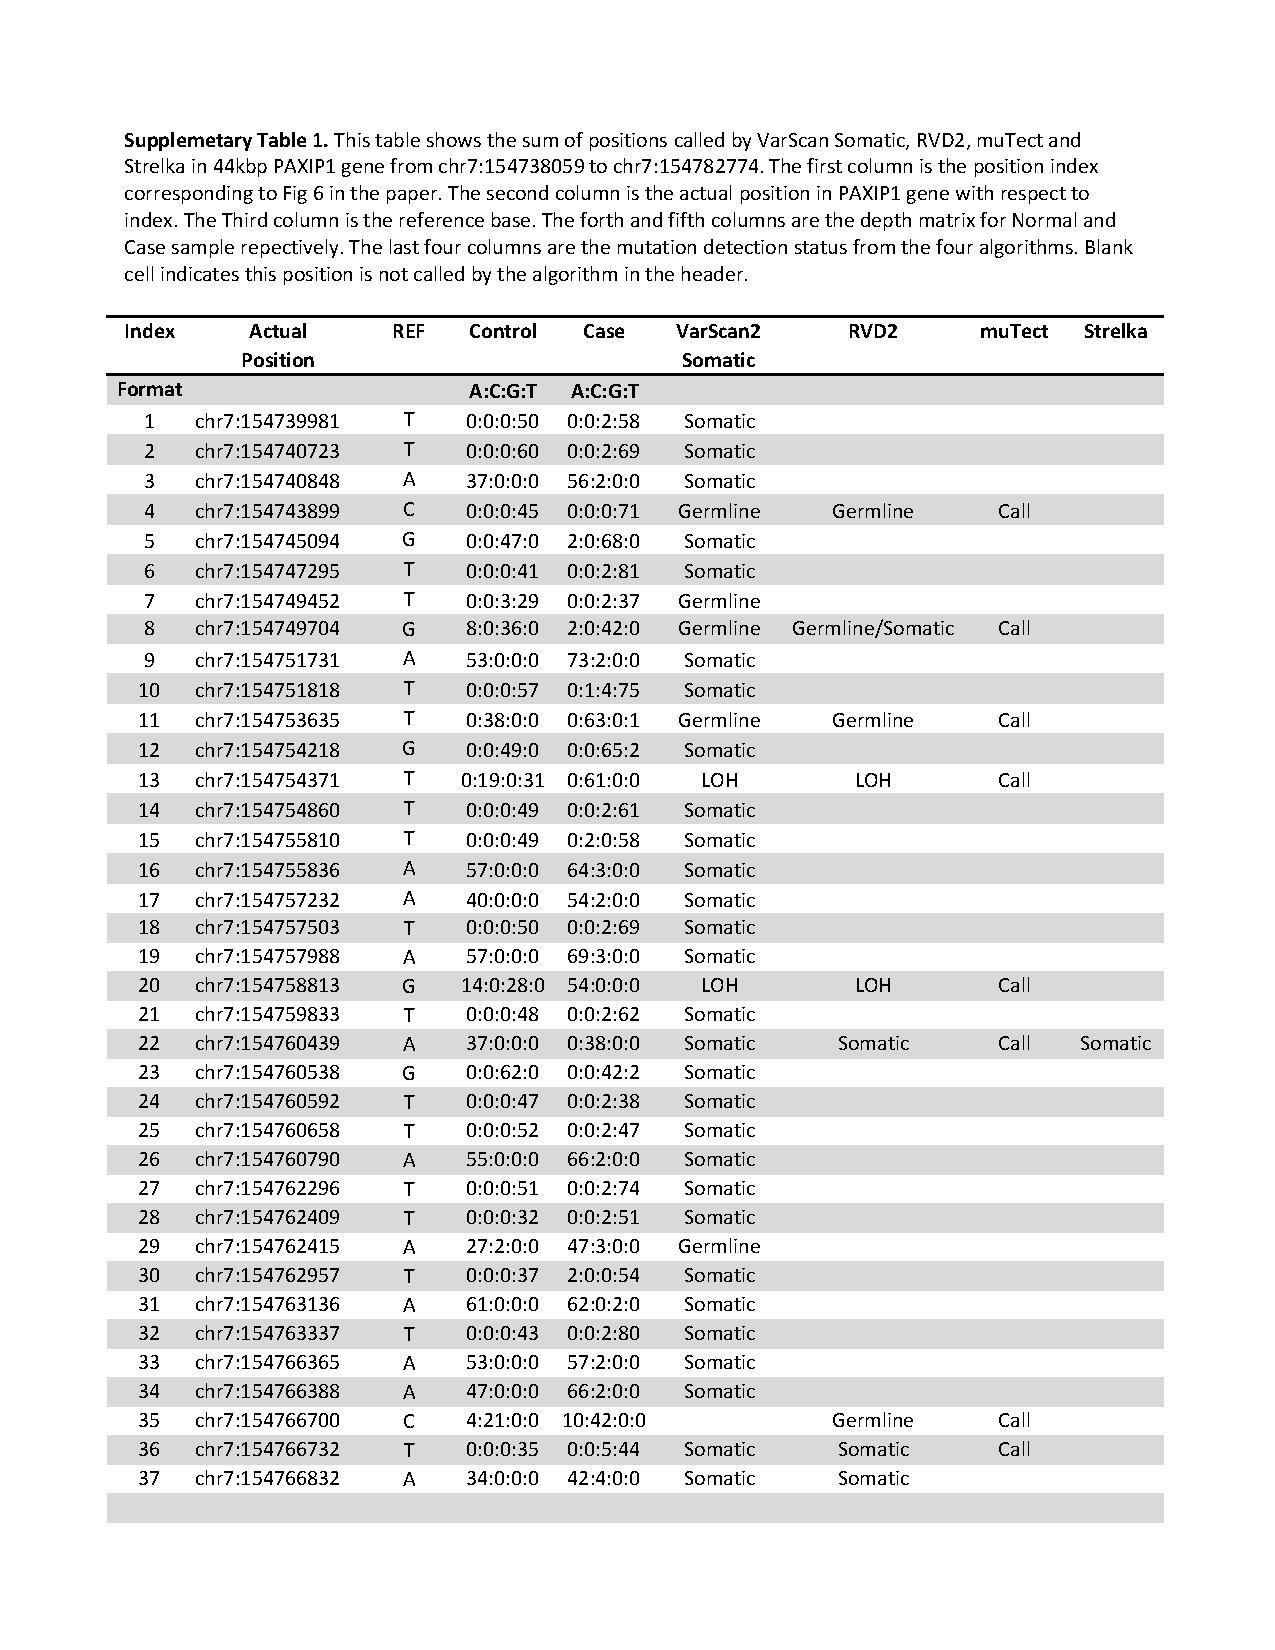
\includepdf[pages={1-},scale=1]{pdf_figs/position_lookup_chart_all.pdf}

\bibliographystyle{natbib}
\bibliography{bioinfo}
\end{document}
